\likechapter{Приложение А}

\renewcommand{\thetable}{\textmd{A.}\arabic{table}}
\setcounter{table}{0}
\begin{table}[ht!]
	\small
    \caption{Классификация неровностей поверхности и рельефа \cite{mlyavaya}.}
    \label{table_z0}
	\setlength{\extrarowheight}{0.5mm}
	\centering
    \begin{tabular}{|M{0.03\textwidth}|M{0.5\textwidth}|M{0.18\textwidth}|M{0.18\textwidth}|}
    \hline № & Вид поверхности & Класс неровности рельефа K & Размер шероховатости $Z_0$ \\
    
    \hline 1. & Водная поверхность (море, озеро); снежная поверхность & 0 & \makecell{0,02 см \\ 0,05-0,1 см} \\
    
    \hline 2. & Полностью открытый рельеф с гладкой поверхностью (взлетные полосы, ровные поля, скошенная трава) & 
    	0,5 & 0,24-0,5 см \\
    
    \hline 3. & Открытые области с небольшими лесозащитными полосами (равнины или небольшие холмы, пашня, травяные 
    	поля); небольшие фермерские постройки, отдельно стоящие деревья или кустарники & 1 & 1-3 см \\
    
    \hline 4. & Ровная, слегка холмистая местность, сельскохозяйственные угодья (поле с высокой растительностью, 
    	пшеничное поле) с несколькими зданиями и навесами высотой до 8 м, расположенными друг от друга на расстоянии 
    	около 1250 м & 0 & 5 см\\
    
    \hline 5. & Ровная или слегка холмистая территория, хозяйственные земли с разбросанными областями построек и 
    	небольшими лесозащитными полосами, среднее расстояние между которыми составляет 1000 м & 2 & 10 см \\
    
    \hline 6. & Сельскохозяйственные угодья с большим количеством зданий или навесами высотой до 8 м, с деревьями, 
    	кустарниками, расположенными друг от друга на расстоянии около 250 м & 2,5 & 20-25 см \\
    
    \hline 7. & Территории с очень неровным рельефом, городские застройки, леса или сельскохозяйственные земли с 
    	многочисленными близкорасположенными лесозащитными полосами, среднее расстояние между которыми составляет 
    	несколько сотен метров; болота с растительностью 
    	& 3 & \makecell{40 см \\ 60 см} \\

    \hline 8. & Города с высокими зданиями & 3,5 & 80-150 см \\
    
    \hline 9. & Большие города, мегаполисы с высокими зданиями и небоскребами & 4 & 160-200 см \\

    \hline
    \end{tabular}
\end{table}

\clearpage

\likechapter{Приложение Б}

\renewcommand{\thetable}{\textmd{Б.}\arabic{table}}
\setcounter{table}{0}
\begin{table}[ht]
    \small
    \caption{Основные характеристики радионуклидов, образующися в топливе.}
    \label{table_tvel_radio}
    \setlength{\extrarowheight}{0.5mm}
    \centering
    \begin{tabular}{|M{0.225\textwidth}|M{0.225\textwidth}|M{0.225\textwidth}|M{0.225\textwidth}|}
    \hline Нуклид & $A_{i}^{0}$, Бк/кг & $Z_i$ & $\gamma_{i}$ \\

    \hline I-131 & $3,000 \times 10^6$ & $6,0$ & $2,88 \times 10^{-2}$ \\
    \hline I-132 & $2,072 \times 10^6$ & $1,0$ & $1,15 \times 10^{-2}$ \\ 
    \hline I-133 & $6,290 \times 10^5$ & $1,0$ & $6,70 \times 10^{-2}$ \\
    \hline I-134 & $3,700 \times 10^6$ & $1,0$ & $3,93 \times 10^{-2}$ \\
    \hline I-135 & $1,590 \times 10^6$ & $1,0$ & $6,28 \times 10^{-2}$ \\

    \hline Cs-134 & $7,770 \times 10^2$ & $1,0$ & $7,71 \times 10^{-8}$ \\
    \hline Cs-137 & $1,600 \times 10^4$ & $1,0$ & $6,23 \times 10^{-2}$ \\
    \hline Cs-138 & $4,100 \times 10^5$ & $0,2$ & Продукт распада Xe-138 \\

    \hline Rb-88 & $4,100 \times 10^5$ & $4,0$ & Продукт распада Kr-88 \\

    \hline Xe-133 & $2,500 \times 10^5$ & $19,0$ & $6,70 \times 10^{-2}$ \\
    \hline Xe-135 & $2,738 \times 10^6$ & $1,0$ & $2,68 \times 10^{-3}$ \\
    \hline Xe-137 & $1,406 \times 10^6$ & $1,0$ & $7,74 \times 10^{-2}$ \\
    \hline Xe-138 & $1,600 \times 10^5$ & $3,0$ & $1,20 \times 10^{-2}$ \\
    
    \hline Kr-85 & $2,500 \times 10^5$ & $1,0$ & $1,30 \times 10^{-2}$ \\
    \hline Kr-87 & $7,030 \times 10^5$ & $1,0$ & $3,64 \times 10^{-2}$ \\
    \hline Kr-88 & $1,600 \times 10^5$ & $4,0$ & $3,64 \times 10^{-2}$ \\

    \hline H-3 & $3,700 \times 10^7$ & $1,0$ & $1,70 \times 10^{-9}$ \\
    \hline
    \end{tabular}
\end{table}

\clearpage

\likechapter{Приложение В}

\renewcommand{\thefigure}{\textmd{В.}\arabic{figure}}
\setcounter{figure}{0}

\begin{figure}[ht]
\centering
    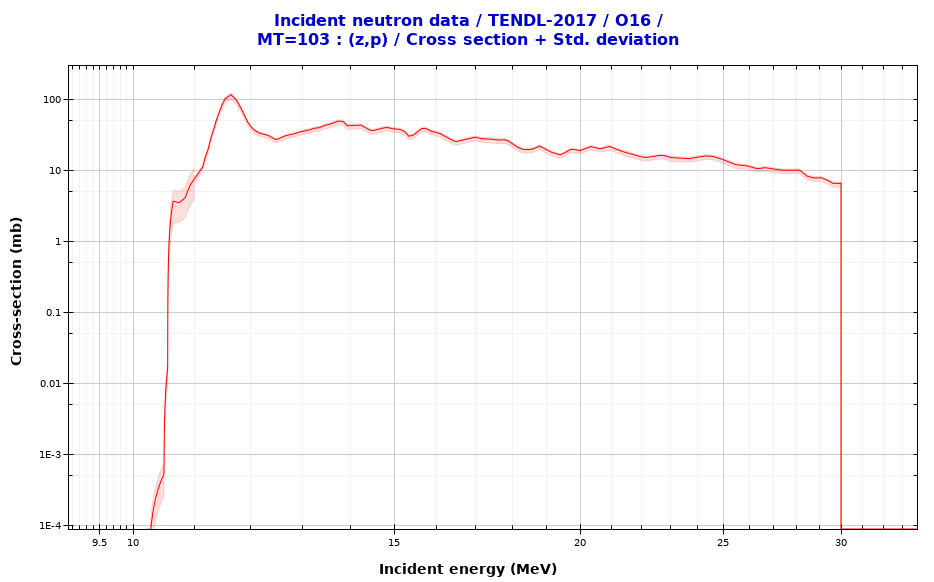
\includegraphics[height=7.9cm]{O16_np_cross}
    \captionsetup{justification=centering}
    \caption{Энергетическая зависимость микроскопического сечения реакции (n, p) на ядре $^{16}\text{O}$ \cite{janis}.}
    \label{fig_O16_cross}
\end{figure}

\begin{figure}[ht]
\centering
    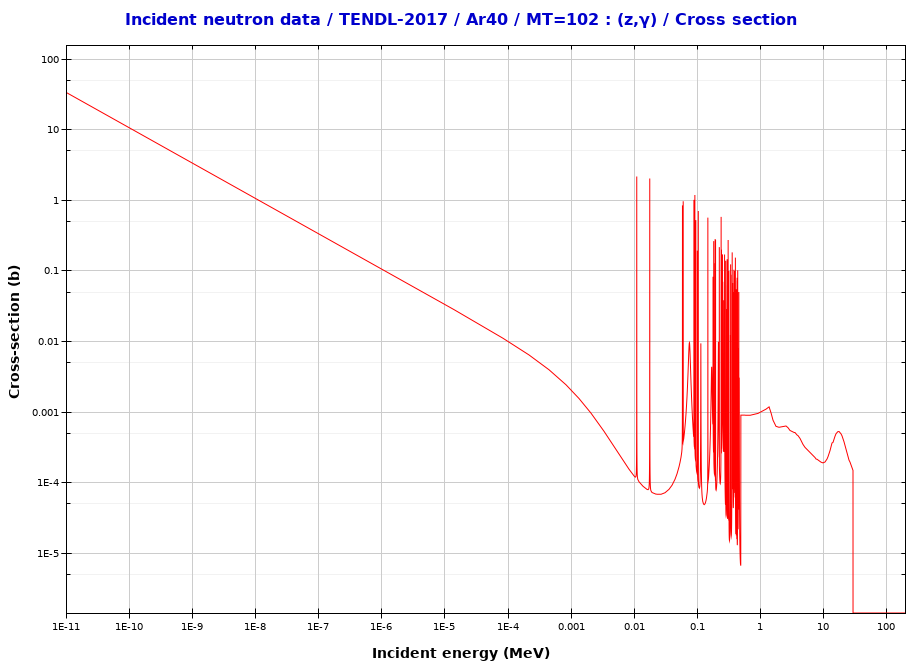
\includegraphics[height=7.9cm]{Ar40_ngamma_cross}
    \captionsetup{justification=centering}
    \caption{Энергетическая зависимость микроскопического сечения реакции (n, $\gamma$) на ядре $^{40}\text{Ar}$ \cite{janis}.}
    \label{fig_Ar40_cross}
\end{figure}

\begin{figure}[ht]
\centering
    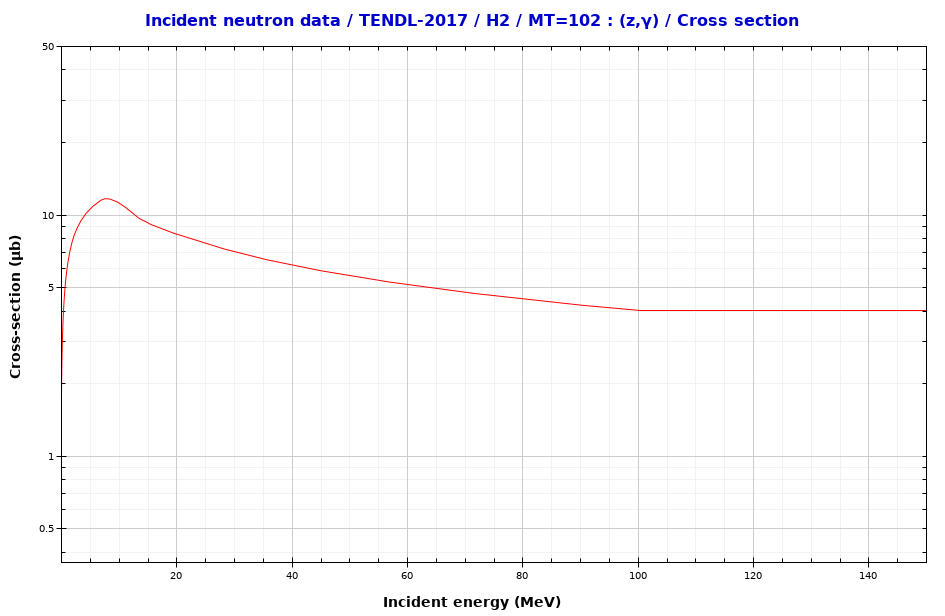
\includegraphics[height=7.9cm]{H2_ngamma_cross}
    \captionsetup{justification=centering}
    \caption{Энергетическая зависимость микроскопического сечения реакции (n, $\gamma$) на ядре $^{2}\text{H}$ \cite{janis}.}
    \label{fig_H2_cross}
\end{figure}

\begin{figure}[ht]
\centering
    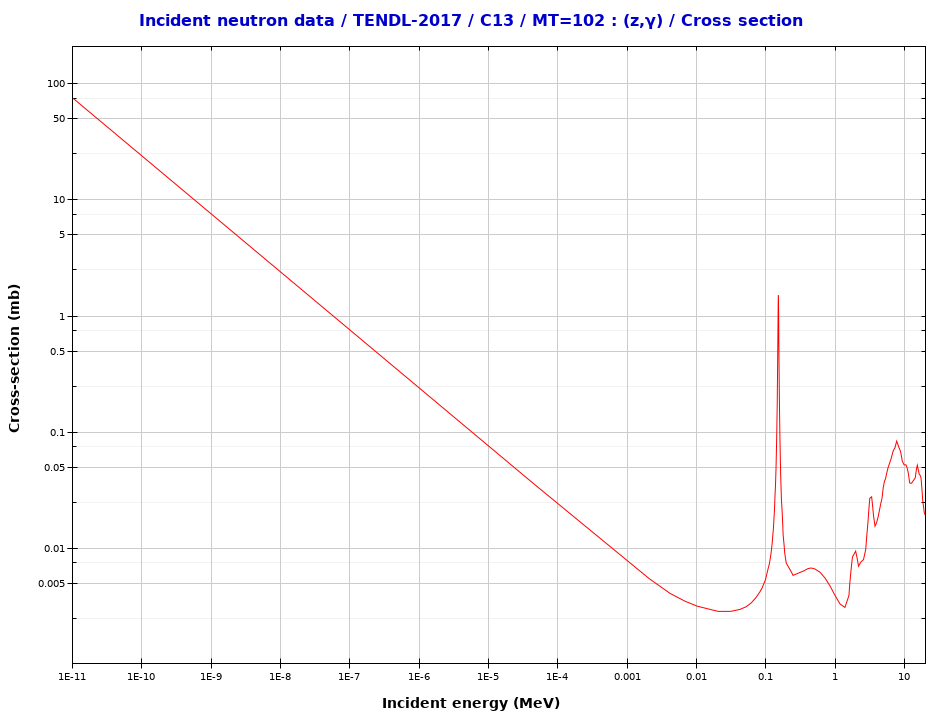
\includegraphics[height=7.9cm]{C13_ngamma_cross}
    \captionsetup{justification=centering}
    \caption{Энергетическая зависимость микроскопического сечения реакции (n, $\gamma$) на ядре $^{13}\text{C}$ \cite{janis}.}
    \label{fig_C13_cross}
\end{figure}

\begin{figure}[ht]
\centering
    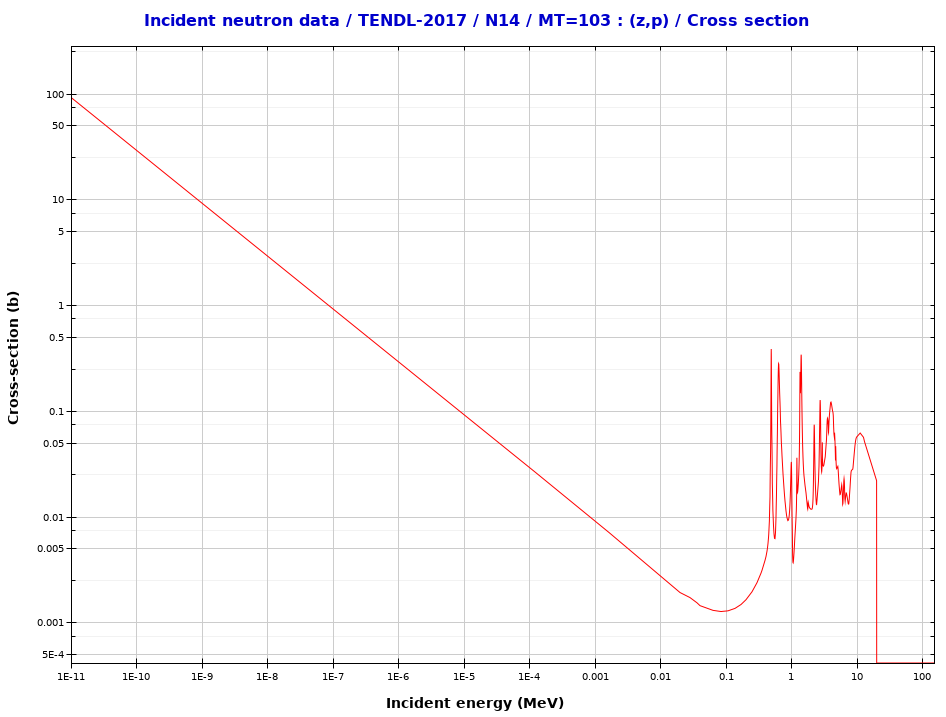
\includegraphics[height=7.9cm]{N14_np_cross}
    \captionsetup{justification=centering}
    \caption{Энергетическая зависимость микроскопического сечения реакции (n, p) на ядре $^{14}\text{N}$ \cite{janis}.}
    \label{fig_N14_cross}
\end{figure}

\begin{figure}[ht]
\centering
    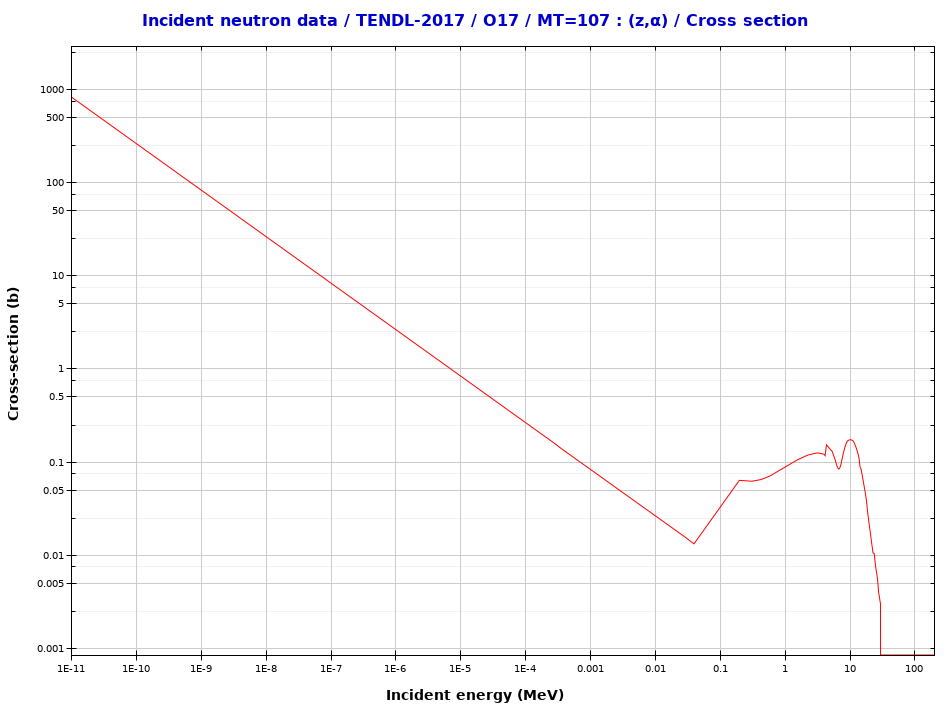
\includegraphics[height=7.9cm]{O17_nalpha_cross}
    \captionsetup{justification=centering}
    \caption{Энергетическая зависимость микроскопического сечения реакции (n, $\alpha$) на ядре $^{17}\text{O}$ \cite{janis}.}
    \label{fig_O17_cross}
\end{figure}

\clearpage

\likechapter{Приложение Г}

\renewcommand{\thetable}{\textmd{Г.}\arabic{table}}
\setcounter{table}{0}
\begin{table}[ht]
    \small
    \caption{Параметры основных радионуклидов, образующихся в теплоносителе первого контура в результате активации 
        нейтронами естественных примесей}
    \label{table_coolant_activ}
    \setlength{\extrarowheight}{1mm}
    \centering

    \newcommand{\colwidth}{0.117}

    \begin{tabular}{|M{\colwidth\textwidth}|M{\colwidth\textwidth}|M{\colwidth\textwidth}|M{\colwidth\textwidth}
        |M{\colwidth\textwidth}|M{\colwidth\textwidth}|M{\colwidth\textwidth}|}
        
        \hline Нуклид & $T_{1/2}$ & Родитель & Реакция & $\sigma^{(2), j}_{i}$, барн & $\sigma^{(1), j}_{i}$, барн & 
            Доля родителя в теплоносителе \\

        \hline $^{16}\text{N}$ & 7,13 секунд & $^{16}\text{O}$ & (n, p) & $0,0$ & $1,0 \times 10^{-29}$ & 1 \\
        \hline $^{41}\text{Ar}$ & 1,83 часов & $^{40}\text{Ar}$ & (n, $\gamma$) & $2,9 \times 10^{-25}$ 
            & $5,2 \times 10^{-27}$ & $7 \times 10^{-6}$ \\
        \hline $^{3}\text{H}$ & 12,32 лет & $^{2}\text{H}$ & (n, $\gamma$) & $2,5 \times 10^{-28}$ 
            & $3,6 \times 10^{-30}$ & $2,3 \times 10^{-2}$ \\
        
        \hline \multirow{3}{*}{$^{14}\text{C}$} & \multirow{3}{*}{5730 лет} & $^{13}\text{C}$ & (n, $\gamma$) 
            & $2,3 \times 10^{-25}$ & $1,5 \times 10^{-27}$ & $5,0 \times 10^{-6}$ \\
        \cline{3-7} & & $^{17}\text{O}$ & (n, $\alpha$) & $2,4 \times 10^{-25}$ & $2,9 \times 10^{-26}$ & $3,7 \times 10^{-2}$ \\
        \cline{3-7} & & $^{14}\text{N}$ & (n, p) & $2,3 \times 10^{-25}$ & $2,0 \times 10^{-26}$ & $2,0 \times 10^{-6}$ \\
        \hline
    \end{tabular}
\end{table}

\clearpage

\likechapter{Приложение Д}
\renewcommand{\thelstlisting}{\textmd{Д.}\arabic{lstlisting}}
\setcounter{lstlisting}{0}

\begin{lstlisting}[caption=Исходный код модуля генерации расчетной сетки и её маркировки, 
                    label={lst_meshgen_all}, basicstyle=\scriptsize]
import os
import sys
from typing import List, Dict

import h5py
import pickle
import meshio
import numpy as np
import pygmsh
from PIL import Image

from config import Config


class Cylinder:
    def __init__(self, radius, height, mesh_size):
        self.radius = radius
        self.height = height
        self.mesh_size = mesh_size


class GmshCylinder:
    def __init__(self, points, circles, circle_ll, lines, surface_ll, surfaces, plane_surfaces, \
        surface_loop, volume):
        self.points = points
        self.circles = circles
        self.circles_ll = circle_ll
        self.lines = lines
        self.surface_ll = surface_ll
        self.surfaces = surfaces
        self.plane_surfaces = plane_surfaces
        self.surface_loop = surface_loop
        self.volume = volume


class MeshGenerator:
    gmsh_cylinders: np.array
    geometry: pygmsh.built_in.Geometry  
    points_2d: np.array 
    points_3d: np.array 
    cells_2d: Dict  
    cells_3d: Dict  
    img_pixels: object
    pix_width: int 
    pix_height: int 
    img_center: List
    radius_pix: int
    radius: int
    scale: float
    phys_coords: np.array
    phys_types: np.array 
    k: np.array 
    marked_points_2d: np.array
    marked_points_3d: np.array

    def __init__(self, config_file):

        self.cfg = Config(config_file)
        self.cfg.init_mesh()
        self.cfg.init_pic()
        self.cfg.init_soft()
        self.cfg.init_koef()
        
        self.__init_cylinders()
        self.__init_image()

        self.coords2pix = lambda coords, w, h: \
            (coords + self.radius) \
            / np.array([2 * self.radius / w, 2 * self.radius / h])

    def __init_cylinders(self):
        self.cylinders = []
        for i in range(len(self.cfg.radius_list)):
            cylinder = Cylinder(
                self.cfg.radius_list[i],
                self.cfg.h,
                self.cfg.step[i]
            )
            self.cylinders.append(cylinder)

    def __init_image(self):
        rgb_img = Image.open(self.cfg.image_path).convert("RGB")
        self.img_pixels = rgb_img.load()
        self.img_pixels_np = np.array(rgb_img)
        self.pix_width = rgb_img.width
        self.pix_height = rgb_img.height
        self.img_center = [int(self.pix_width / 2), int(self.pix_height / 2)]
        self.radius_pix = int(min([self.pix_width, self.pix_height]) / 2)
        self.radius = self.cfg.radius_list[-1]
        self.scale = self.radius / (2 * self.radius_pix)

    def generate_and_save(self):
        self.__generate_mesh()
        self.__save_xml_mesh()
        self.__mark_mesh()
        self.__save_marked_mesh()

    def __get_coords_colors(self, points):
        pix2d = np.zeros([points.shape[0], 2], dtype=np.int)
        pix2d[...] = self.coords2pix(points[:, 0:2], self.pix_width, self.pix_height)[...]
        ixl = np.where(pix2d.T[0] == self.pix_width)[0]
        for ix in ixl:
            pix2d[ix][0] = self.pix_width-1
        iyl = np.where(pix2d.T[1] == self.pix_height)[0]
        for iy in iyl:
            pix2d[iy][1] = self.pix_height - 1

        colors = self.img_pixels_np[pix2d.T[1], pix2d.T[0]]
        return colors

    def __mark_2d_mesh(self):
        self.marked_points_2d["surf_type"][:] = self.cfg.marks[self.cfg.default_mark]
        self.marked_points_2d["z0_position"][:] = 1
        self.marked_points_2d["x"][:] = self.points_2d.T[0]
        self.marked_points_2d["y"][:] = self.points_2d.T[1]
        self.marked_points_2d["z"][:] = self.points_2d.T[2]
        colors2d = self.__get_coords_colors(self.points_2d)
        for k, color in self.cfg.rgb.items():
            indexes = np.where((colors2d[:,0]==color[0]) & (colors2d[:,1]==color[1]) \ 
                & (colors2d[:,2]==color[2]))[0]
            self.marked_points_2d["surf_type"][indexes] = self.cfg.marks[k]

    def __mark_3d_mesh(self):
        self.marked_points_3d["surf_type"][:] = self.cfg.marks[self.cfg.default_mark]
        self.marked_points_3d["x"][:] = self.points_3d.T[0]
        self.marked_points_3d["y"][:] = self.points_3d.T[1]
        self.marked_points_3d["z"][:] = self.points_3d.T[2]

        colors3d = self.__get_coords_colors(self.points_3d)
        for k, color in self.cfg.rgb.items():
            indexes = np.where((colors3d[:,0]==color[0]) & (colors3d[:,1]==color[1]) \ 
                & (colors3d[:,2]==color[2]))[0]
            self.marked_points_3d["surf_type"][indexes] = self.cfg.marks[k]

        self.marked_points_3d["z0_position"][:] = 0
        for k, z0 in self.cfg.z0.items():
            indexes = np.where((self.points_3d.T[2]<=z0) \ 
                & (self.marked_points_3d["surf_type"]==k.encode()))[0]
            self.marked_points_3d["z0_position"][indexes] = 1

        for m in self.cfg.marks.values():
            indexes = np.where(self.marked_points_3d["surf_type"]==m.encode())[0]
            self.marked_points_3d["k"][indexes] = self.cfg.k[m]

        for m in self.cfg.marks.values():
            for atm_type, hmax in self.cfg.H_max_list.items():
                indexes = np.where((self.marked_points_3d["surf_type"] == m.encode()) &
                                   (self.marked_points_3d["z0_position"]==0) &
                                   (self.marked_points_3d["z"]<hmax))[0]
                self.wind_destrib[atm_type][indexes] = (self.marked_points_3d["z"][indexes] \ 
                    /self.cfg.H0)**self.cfg.k[m]
                indexes = np.where((self.marked_points_3d["surf_type"] == m.encode()) &
                                   (self.marked_points_3d["z"]>=hmax))[0]
                self.wind_destrib[atm_type][indexes] = (hmax / self.cfg.H0)**self.cfg.k[m]


    def __generate_mesh(self):
        self.__create_geometry()
        mesh_3d = pygmsh.generate_mesh(self.geometry, remove_faces=True, gmsh_path=self.cfg.gmsh_path, \
            geo_filename="example.geo")
        self.points_3d, self.cells_3d = mesh_3d.points, mesh_3d.cells
        self.__mark_bottom_surface()
        mesh_2d = pygmsh.generate_mesh(self.geometry, remove_faces=True, dim=2, \ 
            gmsh_path=self.cfg.gmsh_path)
        self.points_2d, self.cells_2d = mesh_2d.points, mesh_2d.cells

    def __save_xml_mesh(self):
        meshio.write_points_cells(self.cfg.xml_2d_path, self.points_2d, self.cells_2d)
        meshio.write_points_cells(self.cfg.xml_3d_path, self.points_3d, self.cells_3d)

    def __mark_mesh(self):
        self.marked_points_2d = np.zeros(self.points_2d.shape[0],
                                         dtype=[('x', np.float), ('y', np.float), ('z', np.float), \
                                         ('surf_type', np.str), ('z0_position', np.int)])
        self.marked_points_3d = np.zeros(self.points_3d.shape[0],
                                         dtype=[('x', np.float), ('y', np.float), ('z', np.float), \ 
                                   ('surf_type', np.str), ('z0_position', np.int), ('k', np.float)])
        self.wind_destrib = np.zeros(self.points_3d.shape[0],
                                         dtype=[('A', np.float), ('B', np.float), ('C', np.float), \ 
                                ('D', np.float), ('E', np.float), ('F', np.float), ('G', np.float)])
        self.__mark_2d_mesh()
        self.__mark_3d_mesh()

    def __save_marked_mesh(self):
        ext = os.path.splitext(self.cfg.mesh_path)
        if ext == ".h5":
            with h5py.File(self.cfg.mesh_path, 'w') as f:
                f.create_dataset(name="2D_COORDS", data=self.marked_points_2d)
                f.create_dataset(name="3D_COORDS", data=self.marked_points_3d)
                f.create_dataset(name="WIND", data=self.wind_destrib)
                f.flush()
        else:
            d = {
            "2D_COORDS": self.marked_points_2d,
            "3D_COORDS": self.marked_points_3d,
            "WIND": self.wind_destrib
            }
            with open(self.cfg.mesh_path, "wb") as f:
                pickle.dump(d,f)
                f.flush()

    def __create_geometry(self):
        self.geometry = pygmsh.built_in.Geometry()
        self.gmsh_cylinders = []
        for cylinder in self.cylinders:
            self.gmsh_cylinders.append(
                self.__add_cylinder(cylinder, self.gmsh_cylinders[-1] if len(self.gmsh_cylinders) \ 
                    != 0 else None)
            )

    def __mark_bottom_surface(self):
        bottom_surfaces = [cylinder.plane_surfaces[0] for cylinder in self.gmsh_cylinders]
        center_point = self.gmsh_cylinders[0].points[0]
        self.geometry.add_physical_surface(bottom_surfaces)
        self.geometry.add_physical_point(center_point)

    def __add_cylinder(self, cylinder, prev_cylinder):
        base_coords = [
            np.array([0.0, 0.0, 0.0]),
            np.array([0.0, 0.0, cylinder.height]),
        ]

        coords = [
            np.array([cylinder.radius, 0.0, 0.0]),
            np.array([0.0, cylinder.radius, 0.0]),
            np.array([-cylinder.radius, 0.0, 0.0]),
            np.array([0.0, -cylinder.radius, 0.0]),
            np.array([cylinder.radius, 0.0, cylinder.height]),
            np.array([0.0, cylinder.radius, cylinder.height]),
            np.array([-cylinder.radius, 0.0, cylinder.height]),
            np.array([0.0, -cylinder.radius, cylinder.height])
        ]

        circle_points_idx = [
            np.array([2, 0, 3]),
            np.array([3, 0, 4]),
            np.array([4, 0, 5]),
            np.array([5, 0, 2]),

            np.array([6, 1, 7]),
            np.array([7, 1, 8]),
            np.array([8, 1, 9]),
            np.array([9, 1, 6])
        ]

        circles_line_loop_idx = [
            np.array([0, 1, 2, 3]),
            np.array([4, 5, 6, 7]),
        ]

        line_points_idx = [
            np.array([6, 2]),
            np.array([7, 3]),
            np.array([8, 4]),
            np.array([9, 5]),
        ]

        surfaces_line_loop_idx = [
            np.array([0, 0, 1, 4]),
            np.array([1, 1, 2, 5]),
            np.array([2, 2, 3, 6]),
            np.array([3, 3, 0, 7])
        ]

        points = self.__create_points(base_coords, coords, cylinder.mesh_size, prev_cylinder)
        circles = self.__create_circles(points, circle_points_idx)
        circle_ll = self.__create_circle_line_loops(circles, circles_line_loop_idx)
        lines = self.__create_lines(points, line_points_idx)
        surface_ll = self.__create_surface_line_loops(lines, circles, surfaces_line_loop_idx)
        surfaces = self.__create_surfaces(surface_ll)
        plane_surfaces = self.__create_plane_surfaces(circle_ll, prev_cylinder)
        surface_loop = self.__create_surface_loop(surfaces, plane_surfaces, prev_cylinder)
        volume = self.__create_volume(surface_loop)

        return GmshCylinder(points, circles, circle_ll, lines, surface_ll,
                            surfaces, plane_surfaces, surface_loop, volume)

    def __create_points(self, base_coords, point_coords, lcar, prev_cylinder):
        points = [self.geometry.add_point(point, lcar=lcar) for point in point_coords]
        if prev_cylinder is not None:
            points = [prev_cylinder.points[0], prev_cylinder.points[1]] + points
        else:
            points = [self.geometry.add_point(point, lcar=0.0) for point in base_coords] + points
        return points

    def __create_circles(self, points, circle_points_idx):
        circles = [
            self.geometry.add_circle_arc(points[idx[0]], points[idx[1]], points[idx[2]])
            for idx in circle_points_idx
        ]
        return circles

    def __create_circle_line_loops(self, circles, circle_ll_idx):
        circle_ll = [
            self.geometry.add_line_loop([circles[idx[0]], circles[idx[1]], circles[idx[2]], \
                circles[idx[3]]])
            for idx in circle_ll_idx
        ]
        return circle_ll

    def __create_lines(self, points, line_points_idx):
        lines = [self.geometry.add_line(points[idx[0]], points[idx[1]]) for idx in line_points_idx]
        return lines

    def __create_surface_line_loops(self, lines, circles, surfaces_line_loop_idx):
        surface_line_loops = [
            self.geometry.add_line_loop([lines[idx[0]], circles[idx[1]], -lines[idx[2]], \
                -circles[idx[3]]])
            for idx in surfaces_line_loop_idx
        ]
        return surface_line_loops

    def __create_surfaces(self, surface_line_loops):
        surfaces = [self.geometry.add_surface(surface) for surface in surface_line_loops]
        return surfaces

    def __create_plane_surfaces(self, circle_line_loops, prev_cylinder):
        if prev_cylinder is None:
            plane_surfaces = [self.geometry.add_plane_surface(circle_loop) for circle_loop in \
                circle_line_loops]
        else:
            plane_surfaces = [
                self.geometry.add_plane_surface(circle_loop, [prev_cylinder.circles_ll[i]])
                for i, circle_loop in enumerate(circle_line_loops)
            ]
        return plane_surfaces

    def __create_surface_loop(self, surfaces, plane_surfaces, prev_cylinder):
        if prev_cylinder is None:
            surface_loop = self.geometry.add_surface_loop([plane_surfaces[0], *surfaces, \
                plane_surfaces[1]])
        else:
            surface_loop = self.geometry.add_surface_loop(
                [plane_surfaces[0], *surfaces, plane_surfaces[1], *prev_cylinder.surfaces]
            )
        return surface_loop

    def __create_volume(self, surface_loop):
        volume = self.geometry.add_volume(surface_loop)
        return volume
\end{lstlisting}


\clearpage